\documentclass[a4paper]{article}
\usepackage[utf8]{inputenc}
\usepackage{graphicx}
\usepackage{circuitikz}
\usepackage{placeins}
\usepackage{wrapfig}
\usepackage{siunitx}
\usepackage{hyperref}

\newcommand{\mymeter}[2] 
{  % #1 = name , #2 = rotation angle
\begin{scope}[transform shape,rotate=#2]
\draw[thick] (#1)node(){$\mathbf V$} circle (11pt);
\draw[rotate=45,-latex] (#1)  +(-17pt,0) --+(17pt,0);
\end{scope}
}

\title{Misura della Curva Caratteristica di una Lampadina a Incandescenza}
\author{Giovanni Simionato \and Jia Le Sofia Zheng \and Francesco Giuliano Rossi}
\date{13 Ottobre 2025}

\begin{document}
\maketitle
\section{Introduzione}
In questa esperienza, si voleva misurare la curva caretteristica di una lampadina a incandescenza al variare del potenziale fino al bruciamento della stessa.

\begin{wrapfigure}{r}{0.5\textwidth}
\begin{circuitikz}\label{circuito}
   \draw (0,0) to[ battery1, name=myB ] (0,2)
   to [ resistor ] (3,2)
   to [ bulb ] (3,-1)
   to [ ammeter, mirror ] (0,-1)
   to (0,0)

   (2,1.5) to (3,1.5)
   (2,1.5) to [voltmeter, color=white, name=V1] (2,-0.5)
   to (3,-0.5)

   (4.3,2) to [photodiode, mirror] (4.3,-1)
   to (5.5,-1) 
   to [voltmeter, color=white, name=V2] (5.5,2)
   to (4.3,2);
   
   \ctikztunablearrow{1}{1}{60}{myB}
   \mymeter{V1}{0}
   \mymeter{V2}{0}
\end{circuitikz}
\caption{Circuito usato per V$<$1}
\end{wrapfigure}
A questo scopo, si è costruito un circuito come in figura \ref{circuito}, dove la lampadina e il fotodiodo erano isolati dall'ambiente esterno da un tubo di plastica e nastro isolante nero. Il circuito sulla sinistra è costituito da un alimentatore da laboratorio, una resistenza da $100.4\pm0.1 \Omega$, una lampadina da 6V per 0.300A, e due multimetri. Il circuito sulla destra è costituito da un photodiodo ad alimentazione interna collegato ad un multimetro. 

L'esperimento si è svolto in due fasi. Per tensioni al di sotto di un Volt, si sono tenuti connessi al circuito la resistenza e il fotodiodo. In questo modo si può rilevare il momento in cui la lampadina si illumini, misurando la corrente in uscita dal fotodiodo. La resistenza è stata usata per avere un controllo più fine sul potenziale ai capi della lampadina, dato che la manopola sull'alimentaore non permetteva di avere incrementi abbastanza fini. 
Nella seconda fase, si è scollegata la resistenza e si è tolto il fotodiodo. Il potenziale è stato portato ad un valore inferiore rispetto a quello misurato nella prima fase al potenziale massimo e poi incrementato fino al bruciamento del filamento. 

\newpage
\section{Dati Raccolti e Analisi}
Di seguito rapportiamo tutti i dati raccolti in forma di grafico della corrente rispetto al potenziale. È interessante notare che all'inizio l'andamento è in buona approssimazione lineare come si vede nel prossimo grafico \ref{accensione}\\

\textbf{\huge{COSE DA SCRIVERE}}
\begin{enumerate}
   \item inserire Grafici
   \item analizza curva zoomata e commenti i parametri del fit lineare con errori 
   \item inserire accensione lampadina ovunque
   \item fare fit lineare per I$^2$ vs V con errori
   \item commenti Fotodiodo/Resistenza dinamica
   \item commentare secondo e terzo grafico del comportamento omico che finisce prima dell'accendimento perchè resistevitività cambia per scaldamento filamento
   \item commentiamo buco nel fotodiodo
   \item scrivere nel motivo per cui non saturato fotodiodo che stavamo raggiungendo massima potenza dissipabile da resistenza
\end{enumerate}

\begin{figure}[!htbp]
      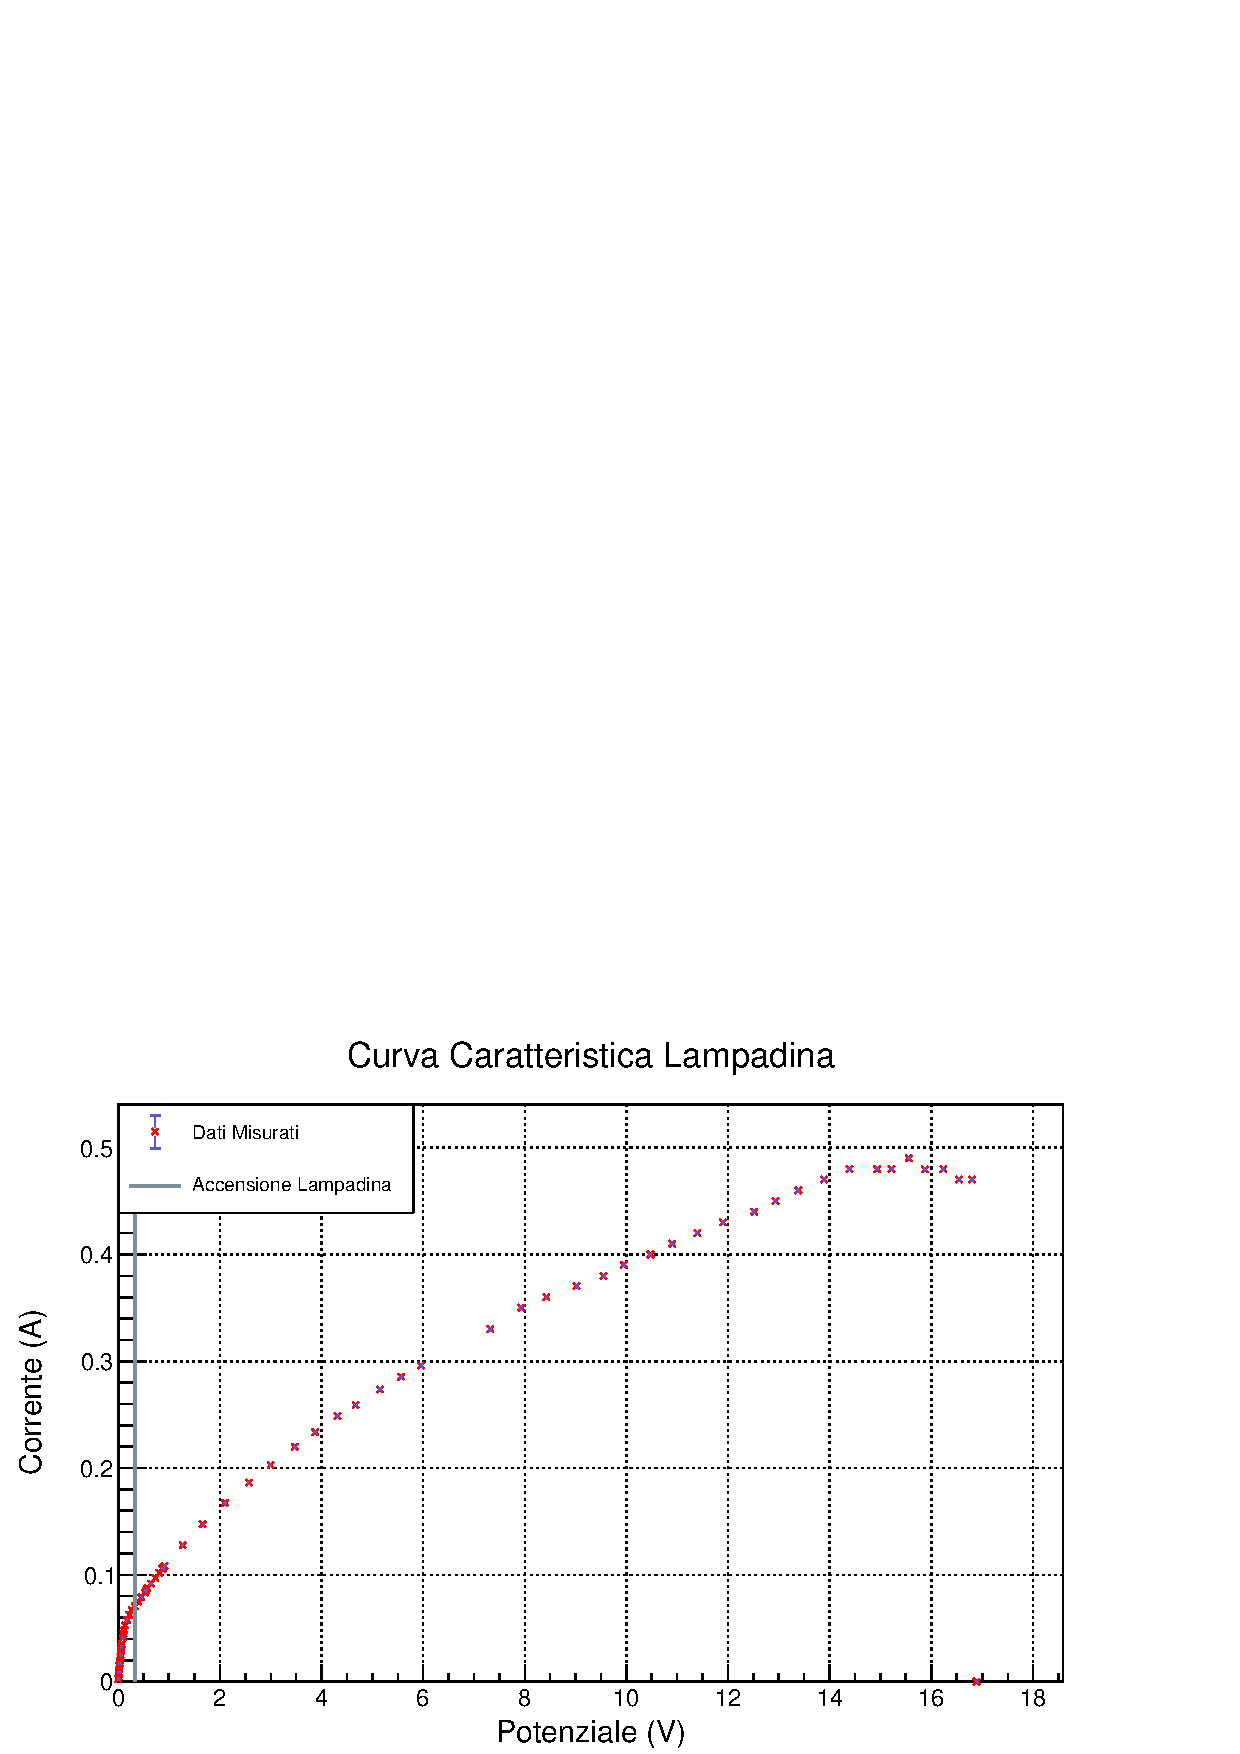
\includegraphics[width=\textwidth]{immagini/bruciarelampa.jpg}
        \caption{Andamento corrente fotodiodo}
\end{figure}
\FloatBarrier

\begin{figure}[!htbp]\label{accensione}
      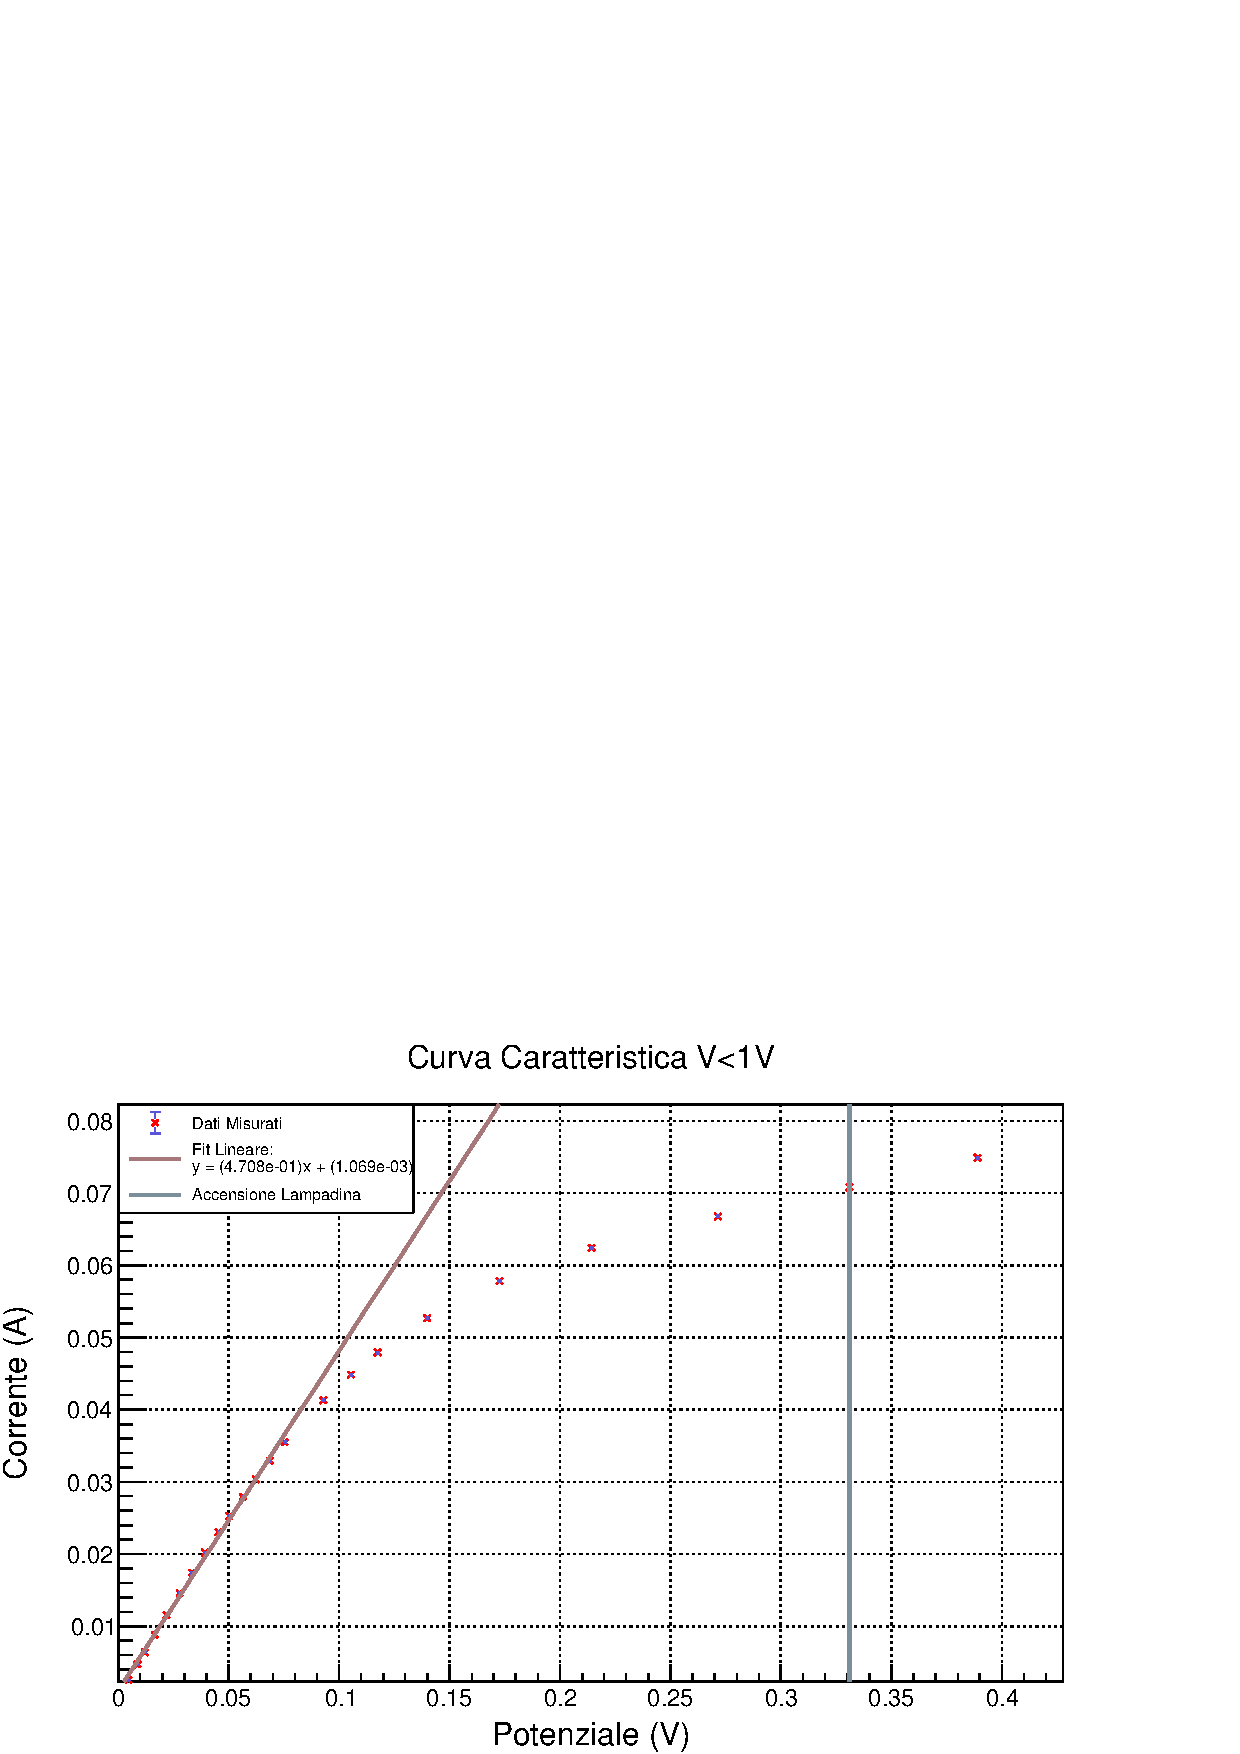
\includegraphics[width=\textwidth]{immagini/graficozoomato1.jpg}
        \caption{Grafico fino all'accensione}
\end{figure}
\FloatBarrier

\begin{figure}[!htbp]
      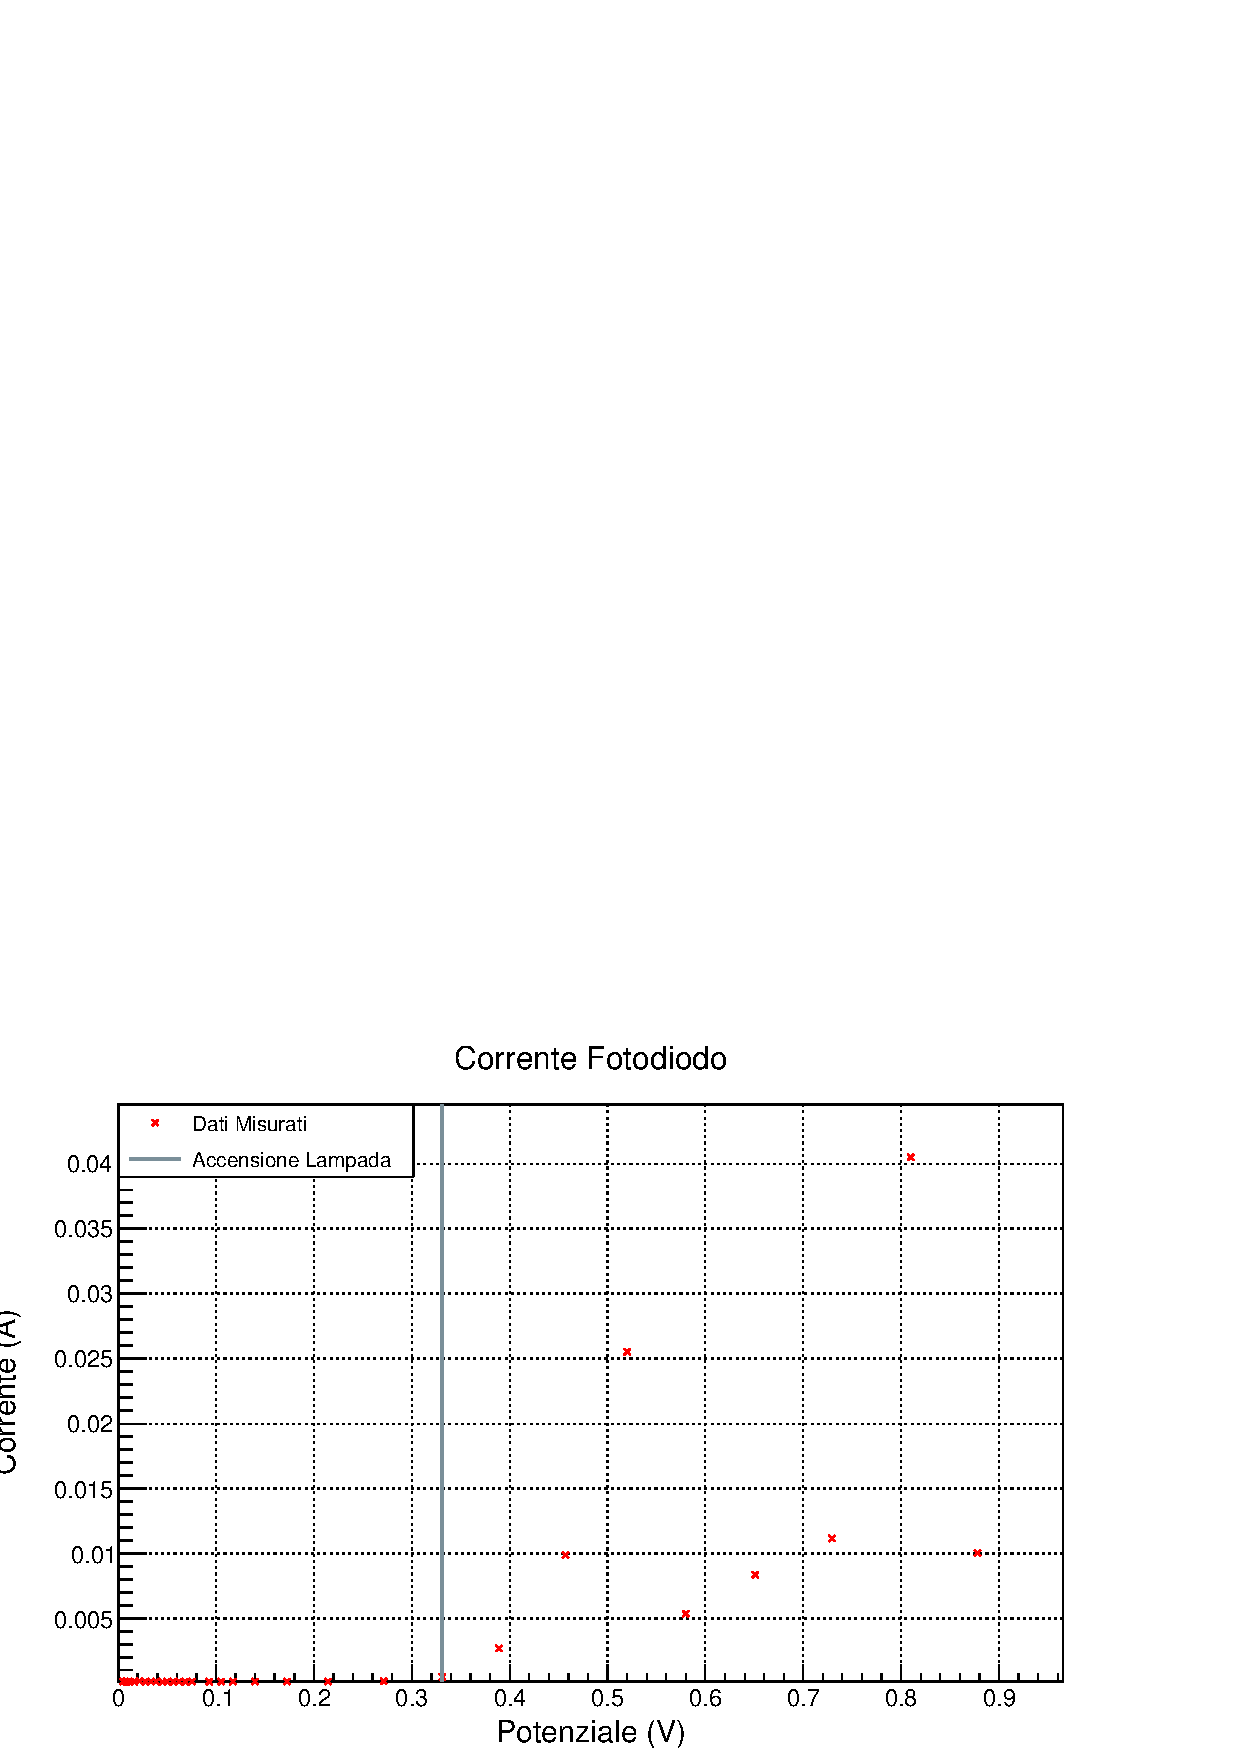
\includegraphics[width=\textwidth]{immagini/fotodiodografico.png}
        \caption{Andamento corrente fotodiodo}
\end{figure}
\FloatBarrier

\begin{figure}[!htbp]
      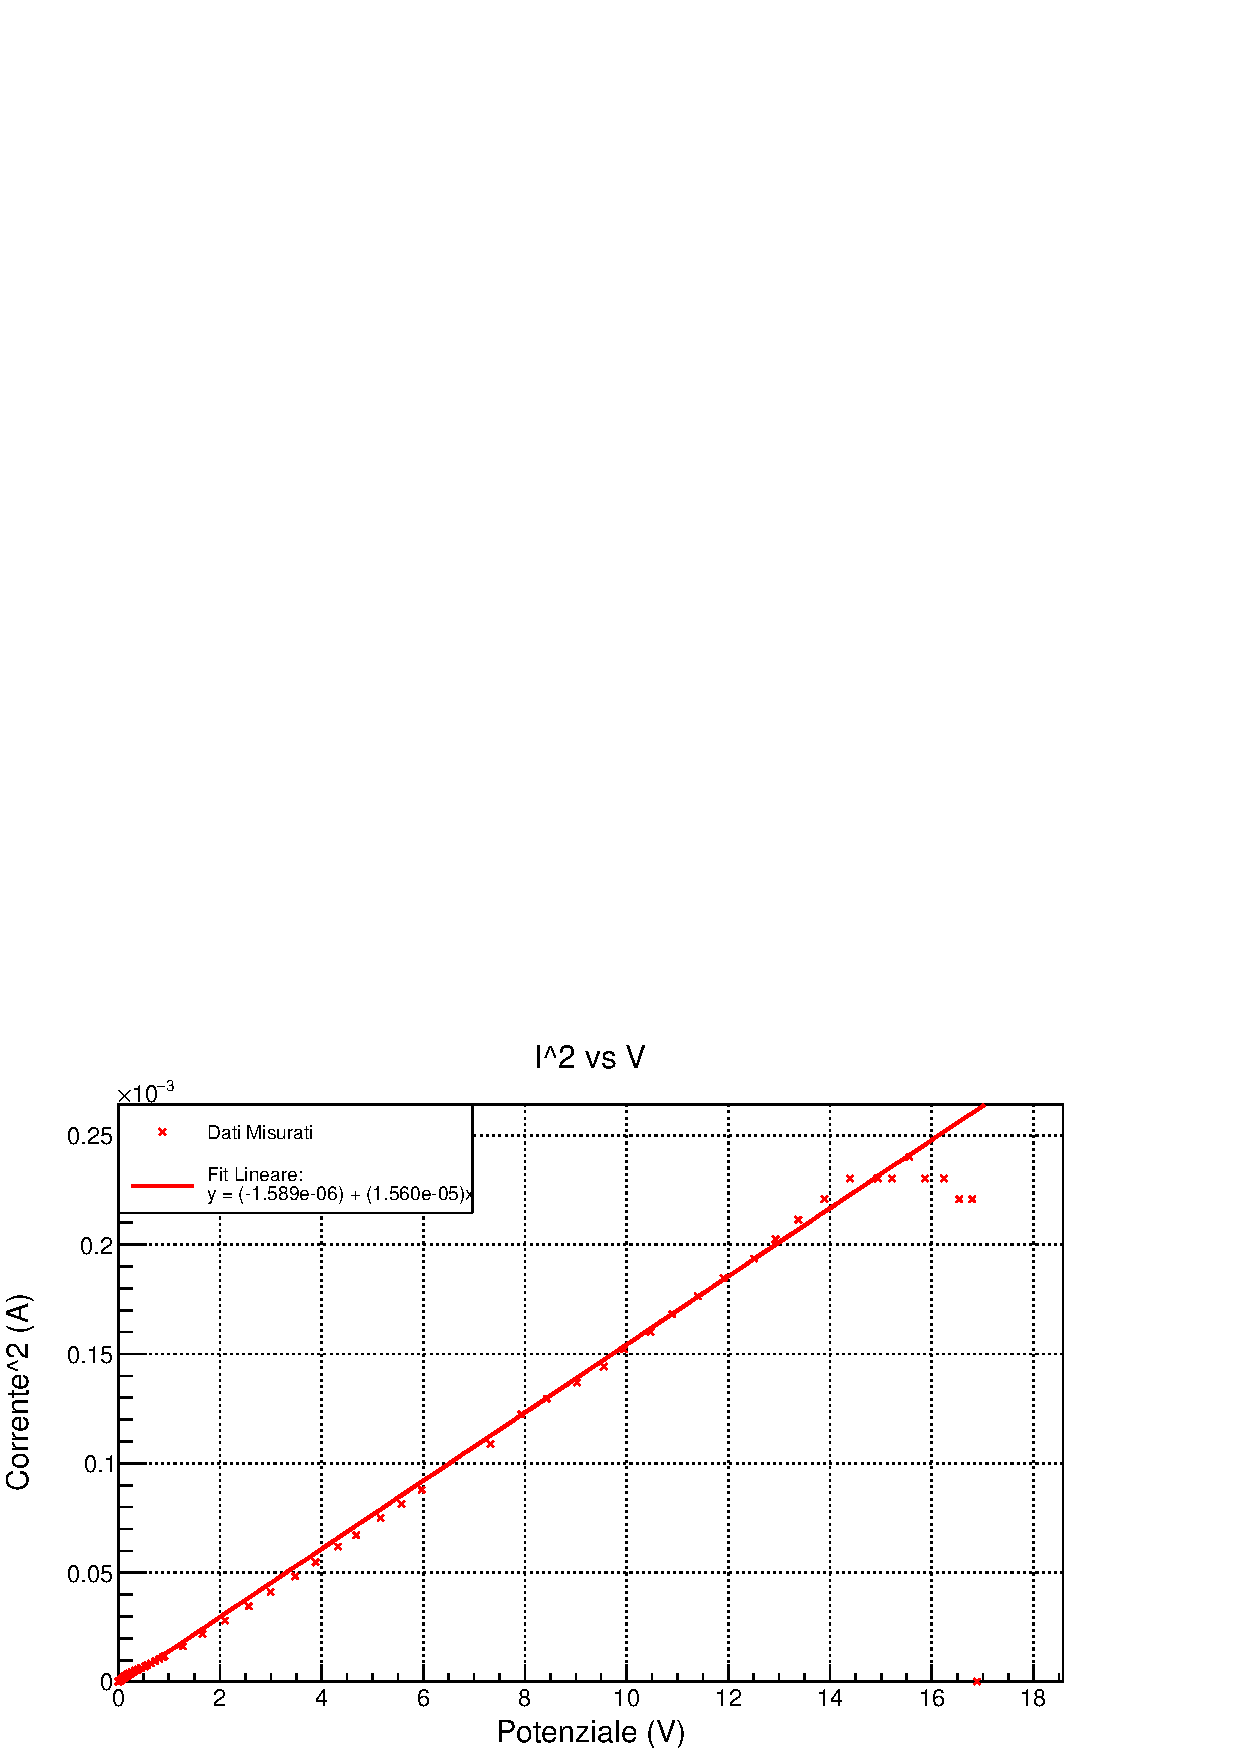
\includegraphics[width=\textwidth]{immagini/I2vsV.png}
        \caption{Curva caratteristica scala semi-quadratica}
\end{figure}
\FloatBarrier

\begin{figure}[!htbp]
      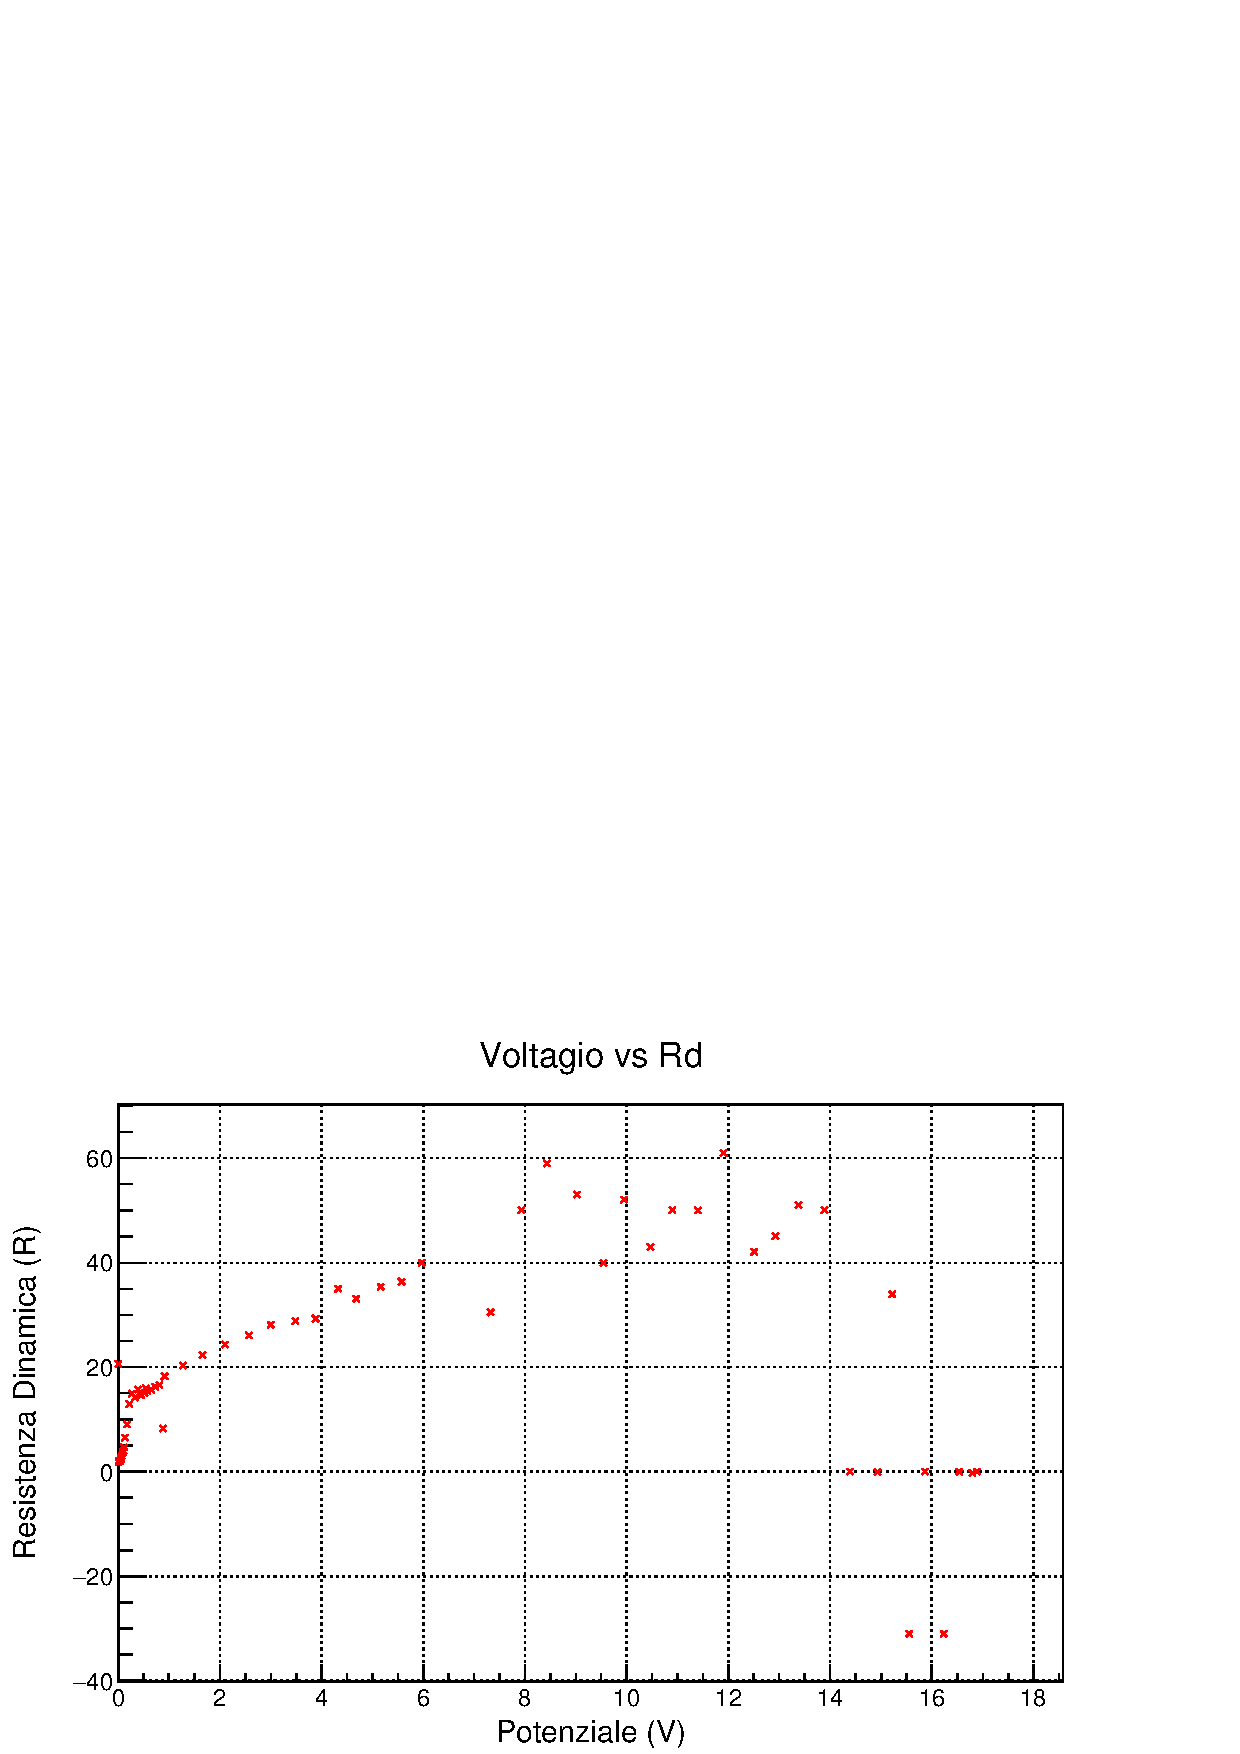
\includegraphics[width=\textwidth]{immagini/fotodiodord.png}
        \caption{Resistenza Dinamica rispetto al potenziale}
\end{figure}
\FloatBarrier



\newpage
\huge{COSE DA SISTEMARE}
FRECCIE SUI MULTIMETRI, INDENT INIZIO SEZIONE, AUMENTA CARATTERE DEGLI ASSI E I PUNTI

\end{document}